\documentclass{article}
\usepackage{tikz}
\usetikzlibrary{calc,arrows}

% https://tex.stackexchange.com/questions/155401/connection-handshake-diagram-with-tikz

\begin{document}

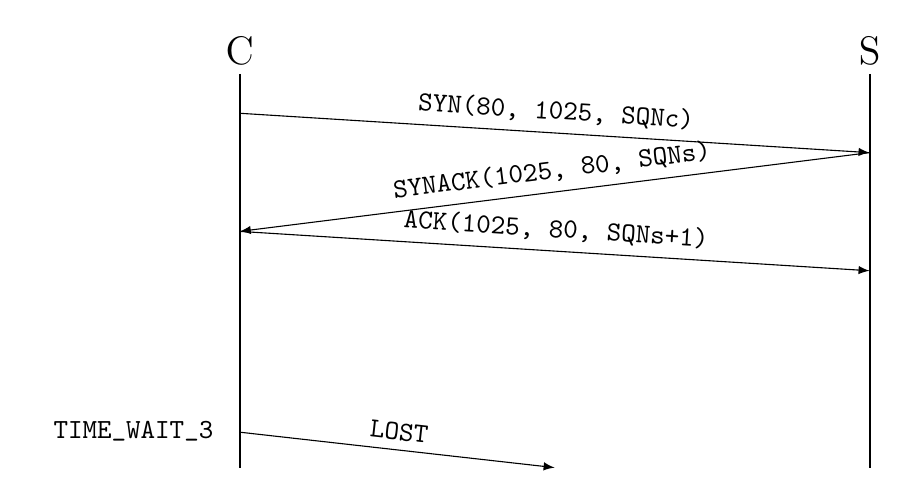
\begin{tikzpicture}[>=latex]	
	\centering
	
	% define the coordinates of client timeline
	\coordinate (A) at (0,5);
	\coordinate (B) at (0,0);
	
	% defien the coordinates of server timeline
	\coordinate (D) at (8,0);
	\coordinate (C) at (8,5);
	
	% draw client and server timeline
	\draw[thick] (A)--(B) (C)--(D);
	% label it on the top	
	\draw (A) node[above]{\Large C};
	\draw (C) node[above]{\Large S};

	\coordinate (E) at ($(A)!.1!(B)$);
	\draw (E) node[left]{
		\begin{tabular}{r}
			%\textit{}\\
			%\verb$$
		\end{tabular}
	};

	\coordinate (F) at ($(C)!.2!(D)$);
	\draw (F) node[right]{
		\begin{tabular}{l}
			%\verb$$\\
			%textit{}
		\end{tabular}
	};	
	\draw[->] (E) -- (F) node[midway,sloped,above]{\verb$SYN(80, 1025, SQNc)$};

	\coordinate (G) at ($(A)!.4!(B)$);
	\draw (G) node[left]{
		\begin{tabular}{l}
			%\verb$$
		\end{tabular}
	};
	\draw[->] (F) -- (G) node[midway,sloped,above]{\verb$SYNACK(1025, 80, SQNs)$};

	\coordinate (H) at ($(C)!.5!(D)$);
	\draw (H) node[right]{
		\begin{tabular}{l}
			%\verb$$
		\end{tabular}
	};
	\draw[->] (G) -- (H) node[midway,sloped,above]{\verb$ACK(1025, 80, SQNs+1)$};

	\coordinate (I) at ($(A)!.7!(B)$);
	\draw (I) node[left]{
		\begin{tabular}{l}
			%\verb$$
		\end{tabular}
	};
	
	\coordinate (K) at ($(I)!.7!(B)$);
	\draw (K) node[left]{
		\begin{tabular}{l}
			\verb$TIME_WAIT_3$
		\end{tabular}
	};
	\coordinate (Mid) at (4,0);
	\draw[->] (K) -- (Mid) node[midway,sloped, above]{\verb$LOST$};
	
\end{tikzpicture}
\end{document} 